\documentclass[tikz,border=2pt]{standalone}
\usepackage{amsmath,amssymb}
\usepackage{tikz}
\usetikzlibrary{arrows.meta}

\begin{document}
% The triangle inequality: going along x and then y is never shorter than going straight.
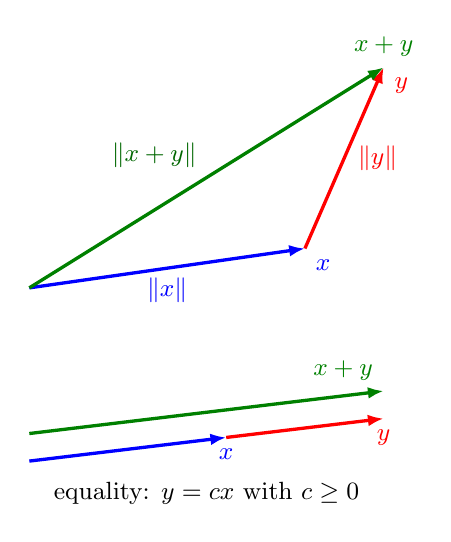
\begin{tikzpicture}[every node/.style={font=\small}, >={Latex[length=2mm]}]
	\draw[->, blue, very thick] (0,0) -- (3.5,0.5) node[below right] {$x$};
	\draw[->, red, very thick] (3.5,0.5) -- (4.5,2.8) node[below right] {$y$};
	\draw[->, green!50!black, very thick] (0,0) -- (4.5,2.8) node[above] {$x+y$};
	\node[blue, below] at (1.75,0.25) {$\|x\|$};
	\node[red, right] at (4.05,1.65) {$\|y\|$};
	\node[green!40!black, above left] at (2.25,1.4) {$\|x+y\|$};
	\begin{scope}[yshift=-2.2cm]
		\draw[->, blue, very thick] (0,0) -- (2.5,0.3) node[below] {$x$};
		\draw[->, red, very thick] (2.5,0.3) -- (4.5,0.54) node[below] {$y$};
		\draw[->, green!50!black, very thick] (0,0.35) -- (4.5,0.89) node[above left] {$x+y$};
		\node[anchor=north] at (2.25,-0.15) {equality: $y=cx$ with $c\ge0$};
	\end{scope}
\end{tikzpicture}
\end{document}
